%xelatex -shell-escape -output-directory=bin ergasia.tex
\documentclass{assignment}

\title{Forecasting Short-Term Time Series using an Artificial Immune System }
\date{Piraeus, 2015}

\author{Vasilis-Thanos Anagnostopoulos}

\begin{document}

\maketitle
% Να σκεφτώ τί αλλαγές θέλω να κάνω με τις αριθμήσεις και άμα θέλω να κάνω.
% Να σκεφτώ να τις ενσωματώσω και στο assignment.cls

\setcounter{page}{1} 
\pagenumbering{roman}

\pagestyle{plain}
\tableofcontents
\listoftables
\listoffigures
\listofalgorithms
%\listoflistings
\newpage

%\pagestyle{headings}
%\pagestyle{fancy}
\setcounter{page}{1} 
\pagenumbering{arabic}

\section{Introduction}

In the following sections, we will review how short-term forecasting in time series can be accomplished using an artificial immune system. In section \ref{ais} we will mention how an artificial immune system works %and in section \ref{time_series} we will mention some general information for time series.
Afterwards we will present our implementation and some results in $CO_2$ measurements.

\section{Artificial Immune Systems}
\label{ais}

The natural immune system is a complex system for the operation of which many publications have been made \cite{wiki:immune_system}. Apart from its ability to fight infections and foreign cells towards the body, it also has a memory, a particularly important property, since memory allows it to identify and manage more directly an invasion by pathogens that have infected the organism in older periods. 

An artificial immune system (AIS) models the ability of the natural immune system of the vertebrates to detect foreign cells in the organism. The result is a new computing model that is capable of recognizing patterns and this new computing model is applied mainly to detect anomalies \cite{engelbrecht,wiki:artificial_immune_system}.

The implementation of an AIS includes a variety of topics such as \cite{engelbrecht,karakasis_thesis}:

\begin{itemize}
\item hybrid structures and algorithms which take into account the mechanisms of the immune system such as the detection of foreign cells with a certain affinity for the storage of informations and reuse of that particular informations.
\item computational algorithms based on the principles of the immune system, such as as distributed processing, the principle of clone selection and the theory of the immune system.
\end{itemize}


Using the above, \textcite{engelbrecht} lists the basic step for creating a basic AIS (see algorithm \ref{algorith:AIS}). 
\begin{algorithm}                        % enter the algorithm environment
\caption{Basic AIS \cite[p. 427]{engelbrecht}}          % give the algorithm a caption
\label{algorith:AIS}                      % and a label for \ref{} commands later in the document
Initialize a set of artificial lymphocytes (ALC) as population $C$ \; 
Determine the antigen patterns as training set $D_T$ \;
\While{some stopping condition(s) not true}{ 
  \For{each antigen pattern $z_p \in D_T$ }{
    Select a subset of ALCs for exposure to $z_p$, as population, $ S \leq C$ \;
    \For{each ALC $x_i \in S$}{
          Calculate the antigen affinity between $z_p,x_i$ \;
    }
    Select a subset of ALCs with the highest calculated antigen affinity as
population $H \leq S$ \;
    Adapt the ALCs in $H$ with some selection method, based on the calculated antigen affinity and/or the network affinity among ALCs in $H$ \;
    Update the stimulation level of each ALC in $H$ \;
  }
}
\end{algorithm}

According to \textcite{engelbrecht} the algorithm is expanded below:
\begin{description}
\item[Initialize $C$ and determining $D_T$:] The population $C$ may be populated from randomly generated artificial lymphocytes\footnote{The lymphocytes is a type of white blood cell which is found on the natural immune system and is responsible for defending the body against infections \cite{wiki:lymphocytes}.} (ACLs) or with ALCs that are initialized with a cross section of the data set to be learned.

\item[Stopping condition for the while:] Most models of AIS have a stopping condition based on the convergence of the population of the population of ACL or after a specified number of iterations.

\item[Selecting a subset $S$ of ALCs:] The subset $S$ can be the entire set of $P$ or a number of randomly selected ALCs from $P$. 

\item[Calculating the antigen affinity:] The antigen affinity is the measurement of similarity or dissimalirity between the ACLs and the antigen patterns.

\item[Selecting a subset of $H$ of ALCs:] In some of the AIS models, the selection of highest affinity ALCs is based on a preset affinity threshold. Thus, the selected subset $H$ can be the entire set $S$, depending on the preset affinity threshold.

\item[Calculating the network affinity:] This is the measurement of affinity between two ALCs. The different measures of network affinity are the same as those for antigen affinity.A preset network affinity threshold determines whether two or more ALCs are linked to form a network.

\item[Adapting the ALCs in subset $H$:] The adaptation of ALCs can be seen as the maturation process of the ALC.

\item[Updating the stimulation of an ALC:] The stimulation level is calculated in different ways in existing AIS models.

\end{description}

According to \textcite{engelbrecht}, several algorithms have been proposed to solve such AIS such as:
\begin{description}

\item[classical view:] of the immune system is that the immune system distinguishes between self and non-self, using lymphocytes produced in the lymphoid organs. These lymphocytes “learn” to bind to antigen.

\item[clonal selection theory:]  where an active B-Cell produces antibodies through a cloning process. The produced clones are also mutated.

\item[network theory:] where the immune system has the ability to distinguish between dangerous and non-dangerous antigen.

\item[danger theory:] where it is assumed that B-Cells form a network. When a B-Cell responds to an antigen, that B-Cell becomes activated and stimulates all other B-Cells to which it is connected in the network.

\end{description}

Artificial immune systems have been successfully applied in many areas, such as the detection of anomalies, in classification of data, in detecting viruses, e.t.c. \cite{wiki:artificial_immune_system, engelbrecht, karakasis_thesis}.

%\section{Time Series}
%\label{time_series}

\section{Implementation}

In this section we present the implementation of the AIS. It was decided the algorithm to be developed using MATLAB\textsuperscript{\textregistered} \cite{MATLAB:2014}. MATLAB\textsuperscript{\textregistered} (MATrix LABoratry) is a high-level and fourth-generation programming language desinged by MathWorks. It allows matrix manipulations, plotting of functions and data, implementation of algorithms, creation of user interfaces, and interfacing with programs written in other languages, including C, C++, Java, Fortran and Python. It is used in many domains such as signal processing and communications, image and video processing, control systems, test and measurement, computational finance, and computational biology \cite{wiki:matlab,MATLAB:2014}.

This algorithm could have been written in a low-level computer language such as C++, which would have freed it from dependency on other software. However, although low-level languages are very powerful and flexible, they are not as conducive to rapid program development or easy implementation of graphical interfaces. Similar with interpreted languages, such as Python, which allow easier program development than low-level languages do, still they do not include all the prepackaged algorithmic and graphical tools in the basic version of MATLAB\textsuperscript{\textregistered}. 

So even though MATLAB\textsuperscript{\textregistered} is only available commercially, it is commonly used in research, and the advantages that offers overcome the disadvantage of being a commercial product. With MATLAB\textsuperscript{\textregistered} the developed software can be executed in every operating system (Windows, Linux or Mac OS) where MATLAB\textsuperscript{\textregistered} is installed. In a later stage someone could also replace MATLAB\textsuperscript{\textregistered} with GNU Octave\footnote{http://www.gnu.org/software/octave/}.

\subsection{Training the AIS}

The implementation of the AIS was based on the algorithm described by \textcite{AIS_STLF08} (see algorithm \ref{algorith:derek}). 

\begin{algorithm}                        % enter the algorithm environment
\caption{The immune memory creation algorithm \cite{AIS_STLF08}}          % give the algorithm a caption
\label{algorith:derek}                      % and a label for \ref{} commands later in the document
Loading of the training set of antigens \; 
Generation of the initial antibody population \;
Antibody affinity calculation \;
Activated antibody detection and evaluation \;
\While{some stopping condition(s) not true}{ 
	Clonal selection \;
	Clone hypermutation \;
	Antibody affinity calculation \;
	Activated antibody detection and evaluation \;
	Selection of the best antibodies \;
}
\end{algorithm}

The detailed algorithm of the immune memory creation in the proposed model is described below:

\begin{description}
\item[Loading of the training set of antigens:] The whole dataset is divided into two subsets (te\-sting and training ). Immune memory is trained using the training set and the model afterwards is tested using the testing subset \cite{AIS_STLF08}. 

To simplify the our model, we need to preprocessed the dataset in order to get rid of the time series trend and seasonality \cite{AIS_STLF08}. 

If $P_x = [ P_x(1), ... , P_x(n)]$ and $P_y = [ P_y(1), ... , P_y(n)]$ is a vector of the values we want to forecast and a vector of the forecast values accordingly with $n \in \mathbb{N}^+$ being the period of the time series then the input pattern $x = [ x(1), ... , x(n)]$ and the output pattern $y = [ y(1), ... , y(n)]$ presented in our model are vectors with components defined in equation \eqref{eq:x_pattern} and \eqref{eq:y_pattern}:

\begin{equation}
x(i) = \frac{P_x(i)}{\bar{P_x}}
\label{eq:x_pattern}
\end{equation}

\begin{equation}
y(i) = \frac{P_y(i)}{\bar{P_x}}
\label{eq:y_pattern}
\end{equation}

with $ i = 1, ... , n$. The model learns to map $x \rightarrow y$ . Pattern $x$ is presented to the model and the pattern $y$ is obtained as the output of the model. Equation \eqref{eq:y_pattern} is used to receive the forecasted load curve $P_y$ \cite{AIS_STLF08}.

Concatenated patterns x and y form antigens ($AG = [x(1), ... , x(n), y(1), ... , y(n)]$). Thus each antigen is composed of $2 \cdot n$ amino acids with which $P_x(i),P_y(i) \in \mathbb{R}$ and $i \in [1,n]$. It is assumed that the only components of the immune system are antibodies built analogously to antigens. Each antibody has two chains ( x to detect the x-chain of the antigens and y to memorize the y-chain of detected antigens) \cite{AIS_STLF08}.

The task of the immune system is to learn to map a set of antigens into a set of antibodies. For each sub - period of the period (for example if our period is a month, then our sub-period could be each day of the month) the separate immune memory is created using antigens representing only this sub-period (e.g. for forecasting the second day of the month, the AIS learns from antigens which x-chain represents the first day of the month and y-chain represents the second day pattern).  \cite{AIS_STLF08}.

\item[Generation of the initial antibody population:] An initial antibody population is created by copying all the antigens from the training set (antibodies and antigens have the same structure). This way of initialization prevents inserting antibodies in empty regions without antigens \cite{AIS_STLF08}.

\item[Antibody affinity calculation:] The affinity measure is based on the distance between x-chains of antigens and antibodies. The Euclidean distance (see equation \eqref{eq:euclidean_distance})is used \cite{AIS_STLF08}.

\begin{equation}
d = \sqrt{\displaystyle\sum_{i=1}^{n} [x_{Ab}(i) - x_{Ag}(i)]^2}
\label{eq:euclidean_distance}
\end{equation}

where $x_Ab$ and $x_Ag$ are the x-chains of the antibody and antigen, respectively \cite{AIS_STLF08}. Probably more affinity measures can be used and a more thorough search should be done.

\item[Activated antibody detection and evaluation:]  If the affinity of the antibody for the antigen is smaller than or equal to the cross-reactivity threshold $r$, it means that the antigen lies in the antibody recognition region (the antibody is activated by the antigen). For this antibody the forecast error is calculated by equation \eqref{eq:forecast_error} \cite{AIS_STLF08}:

\begin{equation}
d = \frac{1}{n} \cdot \displaystyle\sum_{i=1}^{n} \left| \frac{y_{Ab}(i) - y_{Ag}(i)}{y_{Ag}(i)}\right| \cdot 100\%
\label{eq:forecast_error}
\end{equation}

where $y_{Ab}$ and $y_{Ag}$ are the y-chains of the antibody and antigen activating this antibody.
If several antigens lie in the antibody recognition region, the error is calculated for each of them. The mean error $\bar{\delta}$ is applied to evaluate the antibody and is minimized in the following iterations of the algorithm \cite{AIS_STLF08}.

\item[Stopping condition(s):]  The algorithm stops if the maximum number of iteration $L$  is reached \cite{AIS_STLF08} or the population of antigens does not change (in two consecutive iterations the populations of the antigens remains the same) or there is not even one enable antigens. In the last case the AIS failed and the forecast is impossible.

\begin{description}

\item[Clonal selection:] Each antibody secrets as many clones as the antigens that lying in its recognition region. Thus most clones are generated in the dense clusters of antigens \cite{AIS_STLF08}.

\item[Clone hypermutation:] The main goal of hypermutation is to improve the diversity of the immune system in order to effectively recognize new antigens. The hypermutation is realized as follows. Each clone of the antibody is shifted towards different antigen lying in the recognition region of this antibody. The bigger the error $\delta$ for the given antigen is, the bigger shift toward this antigen is. The shift is calculated according to the equation \eqref{eq:x_hypermutation} and \eqref{eq:y_hypermutation} \cite{AIS_STLF08}:

\begin{equation}
x_{Ab}(i) = x_{Ab}(i) + \eta(i)[x_{Ag}(i)-x_{Ab}(i)]
\label{eq:x_hypermutation}
\end{equation}

\begin{equation}
y_{Ab}(i) =y_{Ab}(i) + \eta(i+n)[y_{Ag}(i)-y_{Ab}(i)]
\label{eq:y_hypermutation}
\end{equation}

where $\eta \in (0, 1)$ is a learning coefficient calculated from the hyperbolic tangent sigmoid function from equation \eqref{eq:sigmoid}:

\begin{equation}
\eta(i) = \frac{2}{1+exp[-\beta \cdot \delta \cdot N_i(1,0.1)]} -1
\label{eq:sigmoid}
\end{equation}

where $\beta$ is the shape parameter and $N_i (1, 0.1)$ are the independent normally distributed random numbers with mean 1 and standard deviation 0.1.

Random factor in equation \eqref{eq:sigmoid} is introduced to avoid stagnation of the learning process caused by getting into local minimums of the error function. This type of hypermutation produces new antibodies only in the regions covered by antigens \cite{AIS_STLF08}.

\item[Selection of the best antibodies:] For each antigen from the training set, the set of antibodies activated by this antigen is determined. Only one antibody from this set, with the best evaluation $\delta$ , is selected to the next population. So the clonal expansion, unnecessary in this model, is halted. The maximum number of antibodies in the next population is equal to the number of antigens, but the real number of antibodies is usually smaller because the same antibody could be selected by the several antigens (it depends on the value of the cross-reactivity threshold $r$). Outliers, i.e. antigens lying away from other antigens, is represented by the separate antibodies \cite{AIS_STLF08}. After the selection of the best antibodies the antibodies are re-evaluated again.

\end{description}

\end{description}

\subsection{Forecast}

The forecasting procedure applies the learned immune memory to new antigens consisting only of x-chain. The new antigen is detected by the antibodies with similar x-chains and the y-chain of the antigen is reconstructed from the y-chains of these antibodies \cite{AIS_STLF08}.

The antibodies represent overlapping clusters of similar antigens. In the forecast procedure a new antigen having only x-chain is presented. The $\Omega$ set of antibodies, activated by this antigen, is determined. The y-chain of the input antigen is reconstructed from the y-chains of the antibodies contained in the $\Omega$ set (see equation \eqref{eq:forecast}).

\begin{equation}
\hat{y}_{Ag} = \frac{\displaystyle\sum_{j=1}^{|\Omega|} w_j \cdot y_{Ab}^j(i) }{\displaystyle\sum_{i=1}^{|\Omega|}w_j}
\label{eq:forecast}
\end{equation}


where $w_j \in (0, 1)$ is the weight whose value is dependent on the distance $d_j$ between the input antigen and the j-th antibody from the $\Omega$ set (see equation \eqref{eq:forecast_weight}).

\begin{equation}
w_j = 1 - \frac{d_j}{r}
\label{eq:forecast_weight}
\end{equation}


Antibodies, closer to the antigen, have higher influence on the forecast. If an antigen is not recognized by the antibodies, it means that it represents a new shape, not contained in the training set. In this case the cross-reactivity threshold $r$ is consistently being increased until the antigen is recognized by one or more antibodies. The level of confidence in the forecast in such a case is low and the forecast should be verified \cite{AIS_STLF08}.

The quality criteria of the AIS is the forecast error. For that reason, the training data are used in the forecast and the forecast values are compared to the actual values. The smaller the error, the better the conversion of the AIS. So the RMSE from this procedure is an indication of how well can the AIS predict the values of the existing shapes. As already mention if a new shape is introduced to the AIS then the level of confidence is reduced.

\subsection{Parameters}

In table \ref{table:input_parameters} the input parameters of the algorithm are summarized and in table \ref{table:output_parameters} the output parameters are summarized.

\begin{table}
\begin{center}
  \begin{tabular}{|m{0.20\textwidth}|m{0.75\textwidth}|}
    \hline
    {\bf Parameters} & {\bf Explanation}\\ \hline \hline

	original\_data & the array of input data used for training the AIS. It should be an array with the lines representing the a hole period of measurements  \\ \hline

	threshold & declares the the cross-reactivity threshold r, for which an antigen is activated  \\ \hline

	relax\_threshold & if an antigen does not react the threshold is relax according to this particular percentage  \\ \hline

	max\_iterations & The maximum number of iterations for producing the antibodies \\ \hline

	beta & The shape parameter \\ \hline

	forecast\_data: & The data for which a forecast from the AIS will be done. If left empty then only the next period will be forecasted. \\ \hline

	input\_antibodies & An initial population of antibodies that can be used \\ \hline

	hypermutation & A parameter that instructs the AIS not to produce new antibodies. Should only be used if the antibodies are provided \\ \hline

	diagnostics & If set to true diagnostics messages will be printed  \\ \hline	

\hline \hline
  \end{tabular}
\caption{The input parameters of the algorithm.}
\label{table:input_parameters}
\end{center}
\end{table}

\begin{table}
\begin{center}
  \begin{tabular}{|m{0.20\textwidth}|m{0.75\textwidth}|}
    \hline
    {\bf Parameters} & {\bf Explaination}\\ \hline \hline

	forecast & the forecast values \\ \hline	

	confidence & the confidence of the forecast values. If there is not an antibody that reacts to the values then threshold is relaxed and that is shown in the confidence values that is between 0 and 1 \\ \hline	

	antibodies & the produced antibodies from the AIS \\ \hline	

	iterations & the iterations that the AIS needed \\ \hline	

	total\_time & the total running time of the algorithm \\ \hline	

	forecast\_antigen & the forecast antigens that were used to produce the forecast \\ \hline	

	rmse & the rmse in the original data of the AIS \\ \hline	

	errors & the errors in the training data from which the rmse is produced \\ \hline	

\hline \hline
  \end{tabular}
\caption{The output parameters of the algorithm.}
\label{table:output_parameters}
\end{center}
\end{table}

\section{Case study}

The Mauna Loa Observatory (MLO) is an atmospheric baseline station on Mauna Loa, on the island of Hawaii. MLO is an atmospheric research facility that has been continuously monitoring and collecting data related to atmospheric change since the 1950's and is known especially for the continuous monitoring of atmospheric carbon dioxide ($CO_2$), \cite{wiki:mauna}.

In our case, we will use the monthly $CO_2$ values from the MLO and we will combing them with the AIS, so we could forecast the $C0_2$ values of the next year. 

In a first stage the linear model (see fig. \ref{fig:linear_model}) and the exponential model (see fig. \ref{fig:exponential_model}) were calculated so we could have a comparison model. Afterwards two AIS models (see fig. \ref{fig:ais_model} and \ref{fig:ais_model_0005}) were calculated using two different set of parameters (see table \ref{table:model_parameters} for the parameters).

\begin{figure}
  \centering
  \begin{subfigure}[b]{0.51\textwidth}
     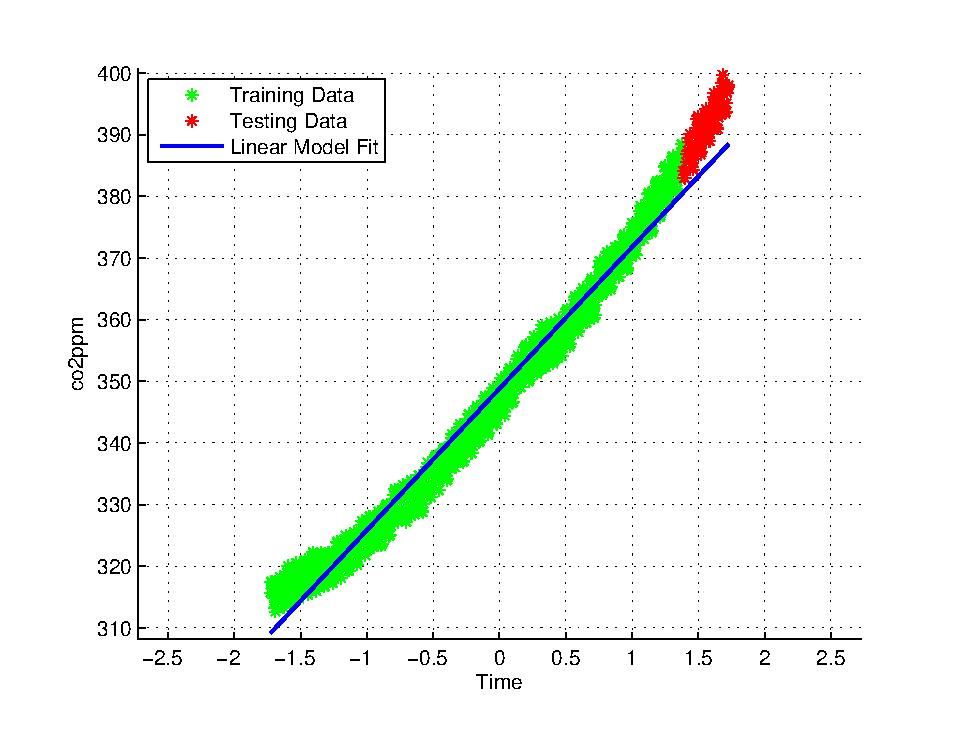
\includegraphics[width=\textwidth]{images/linear_visualization.eps}
  \caption{Visualization of the model}
  \end{subfigure}%
   ~ %add desired spacing between images, e. g. ~, \quad, \qquad, \hfill etc.
  \begin{subfigure}[b]{0.51\textwidth}
    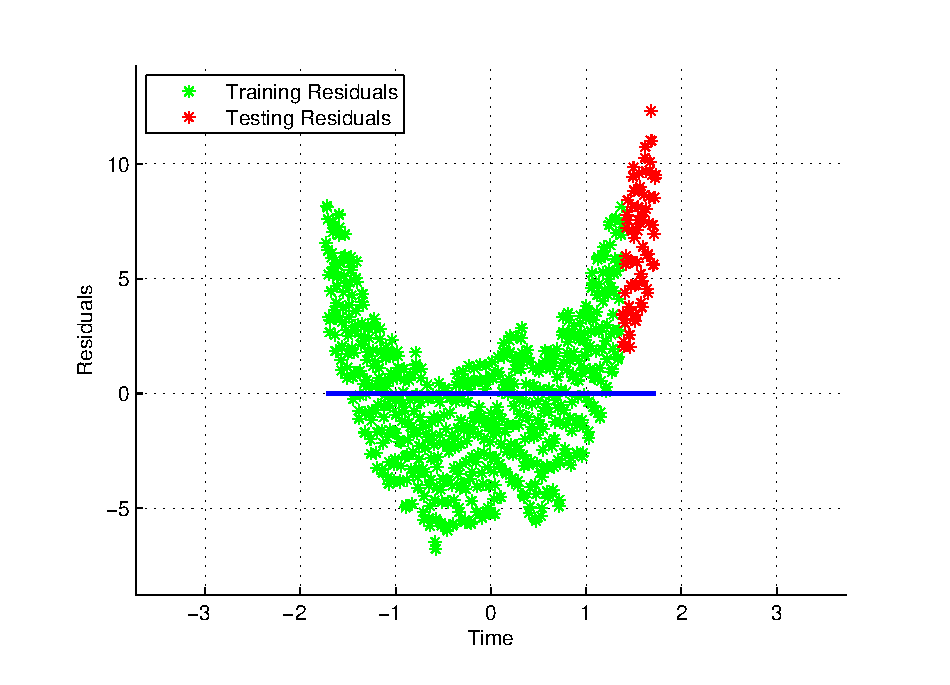
\includegraphics[width=\textwidth]{images/linear_residuals.eps}
  \caption{Visualization of the residuals}
  \end{subfigure}

  \caption{Linear model}
\label{fig:linear_model}
\end{figure}

\begin{figure}
  \centering
  \begin{subfigure}[b]{0.51\textwidth}
     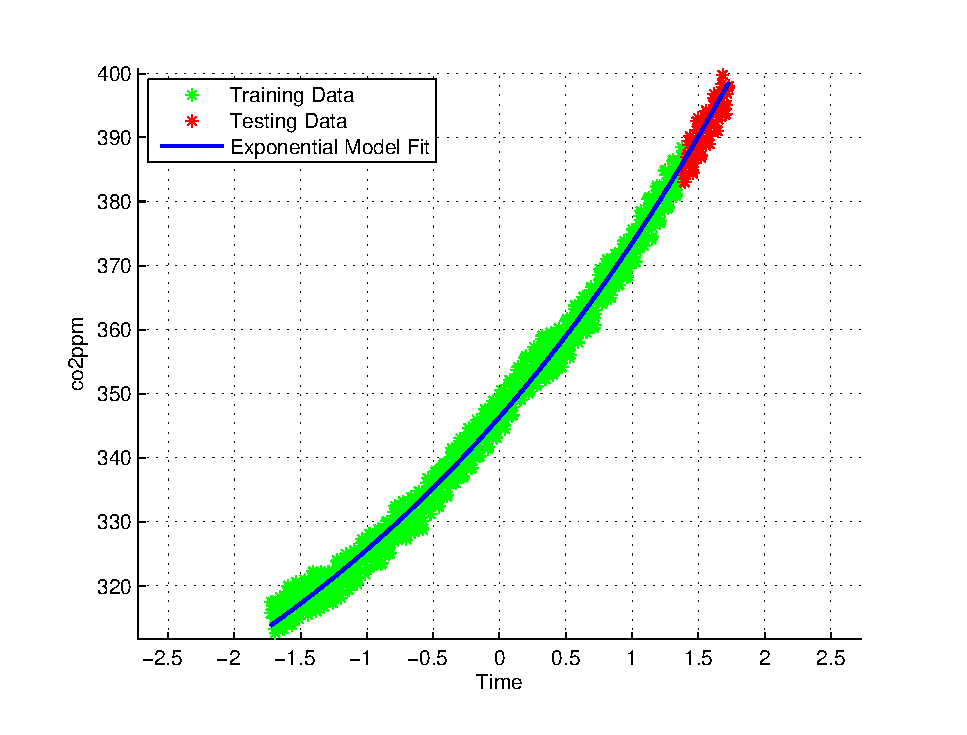
\includegraphics[width=\textwidth]{images/exponential_visualization.eps}
  \caption{Visualization of the model}
  \end{subfigure}%
   ~ %add desired spacing between images, e. g. ~, \quad, \qquad, \hfill etc.
  \begin{subfigure}[b]{0.51\textwidth}
    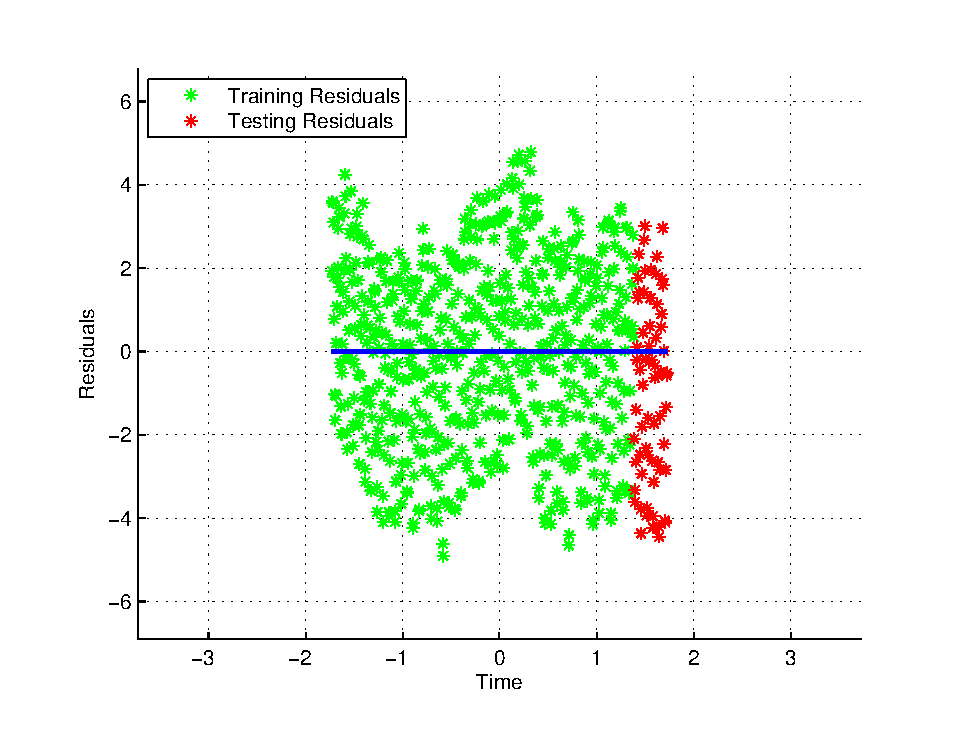
\includegraphics[width=\textwidth]{images/exponential_residuals.eps}
  \caption{Visualization of the residuals}
  \end{subfigure}

  \caption{Exponential model}
\label{fig:exponential_model}
\end{figure}

In all cases the AIS model has lower residuals from the linear and the exponential model. In a latter step, instead of using the values from the previous period to forecast the next period, we used the values from the forecast as input values (orange and yellow lines in the diagrams). In all cases the RMSE error (see table \ref{table:model_parameters}) were better. So the AIS can be used for short and long period forecasts.

\begin{figure}
  \centering
  \begin{subfigure}[b]{0.51\textwidth}
     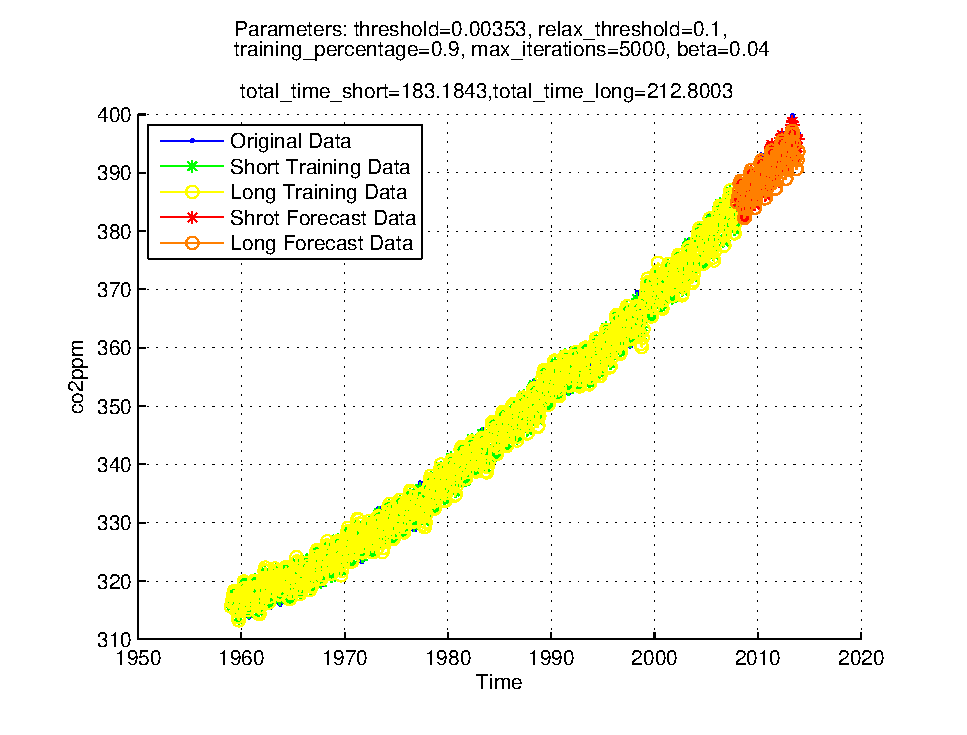
\includegraphics[width=\textwidth]{images/ais_visualization.eps}
  \caption{Visualization of the model}
  \end{subfigure}%
   ~ %add desired spacing between images, e. g. ~, \quad, \qquad, \hfill etc.
  \begin{subfigure}[b]{0.51\textwidth}
    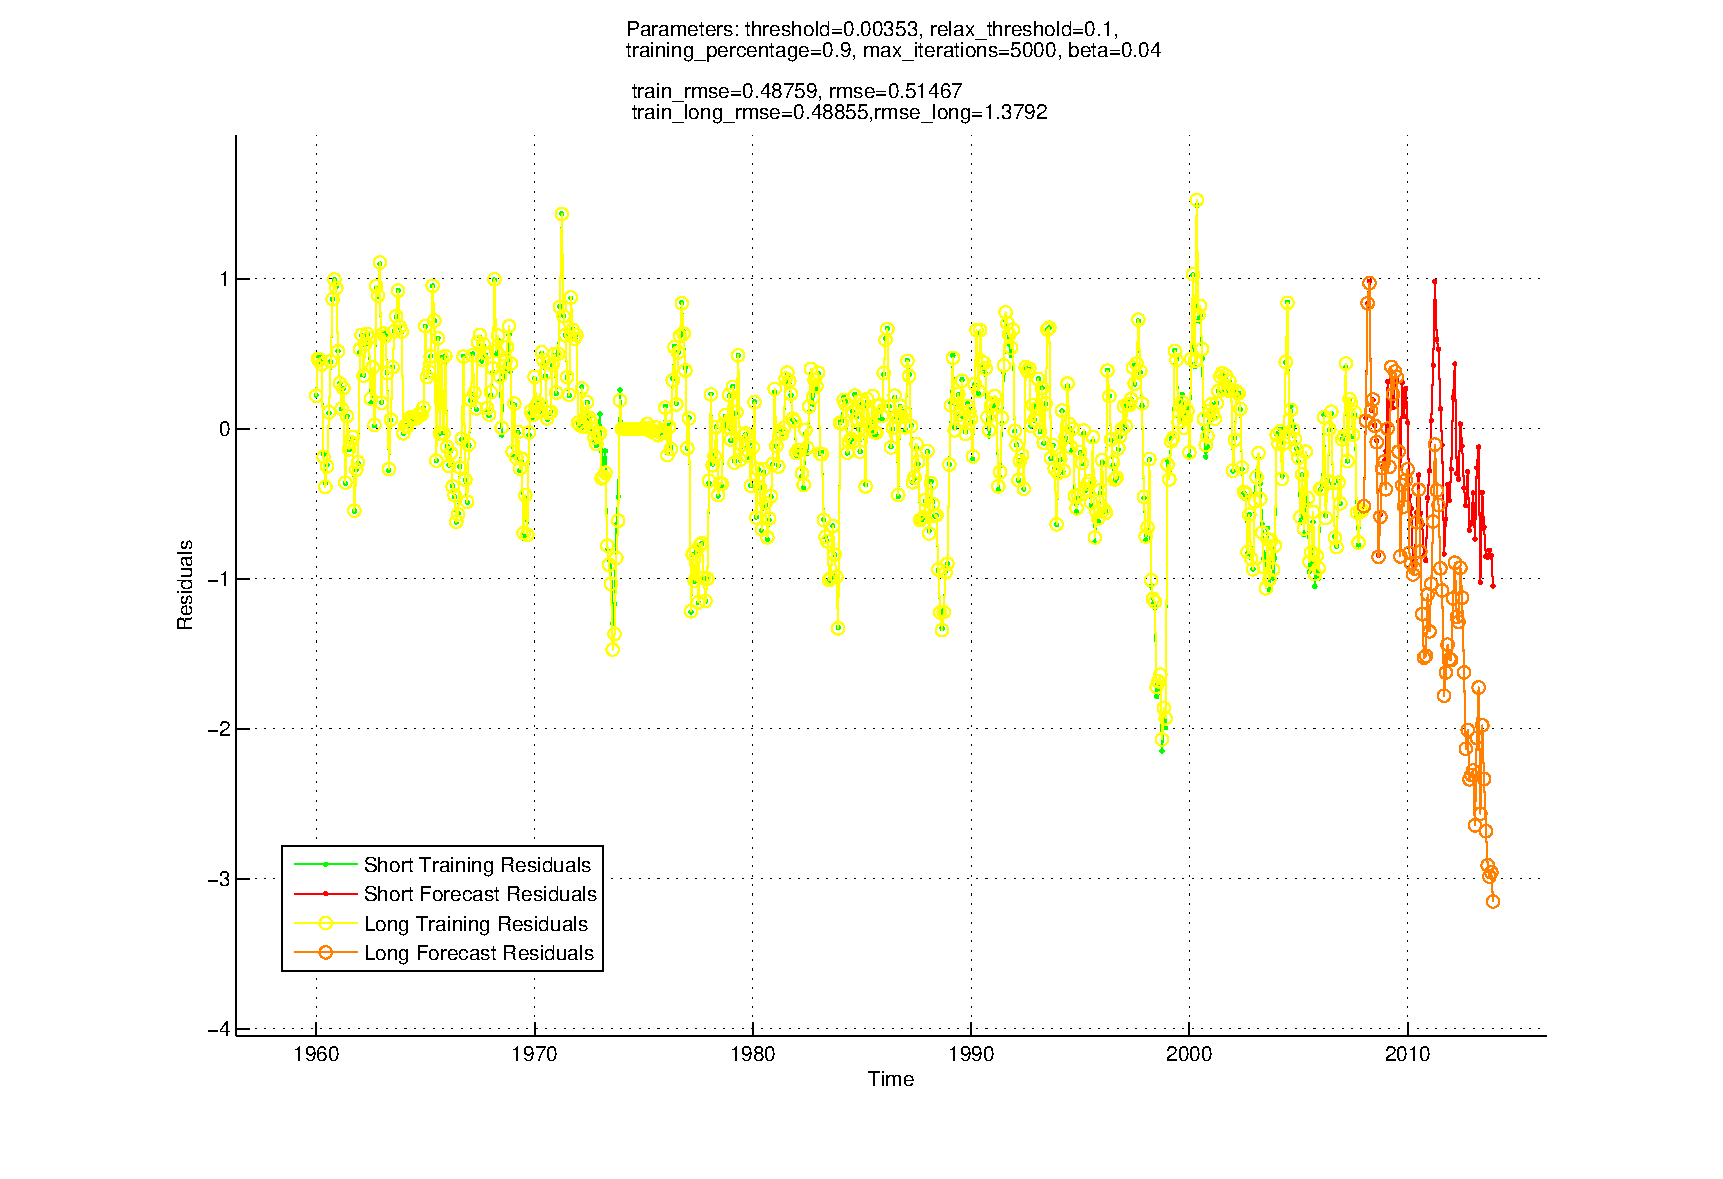
\includegraphics[width=\textwidth]{images/ais_residuals.eps}
  \caption{Visualization of the residuals}
  \end{subfigure}

  \begin{subfigure}[b]{0.51\textwidth}
     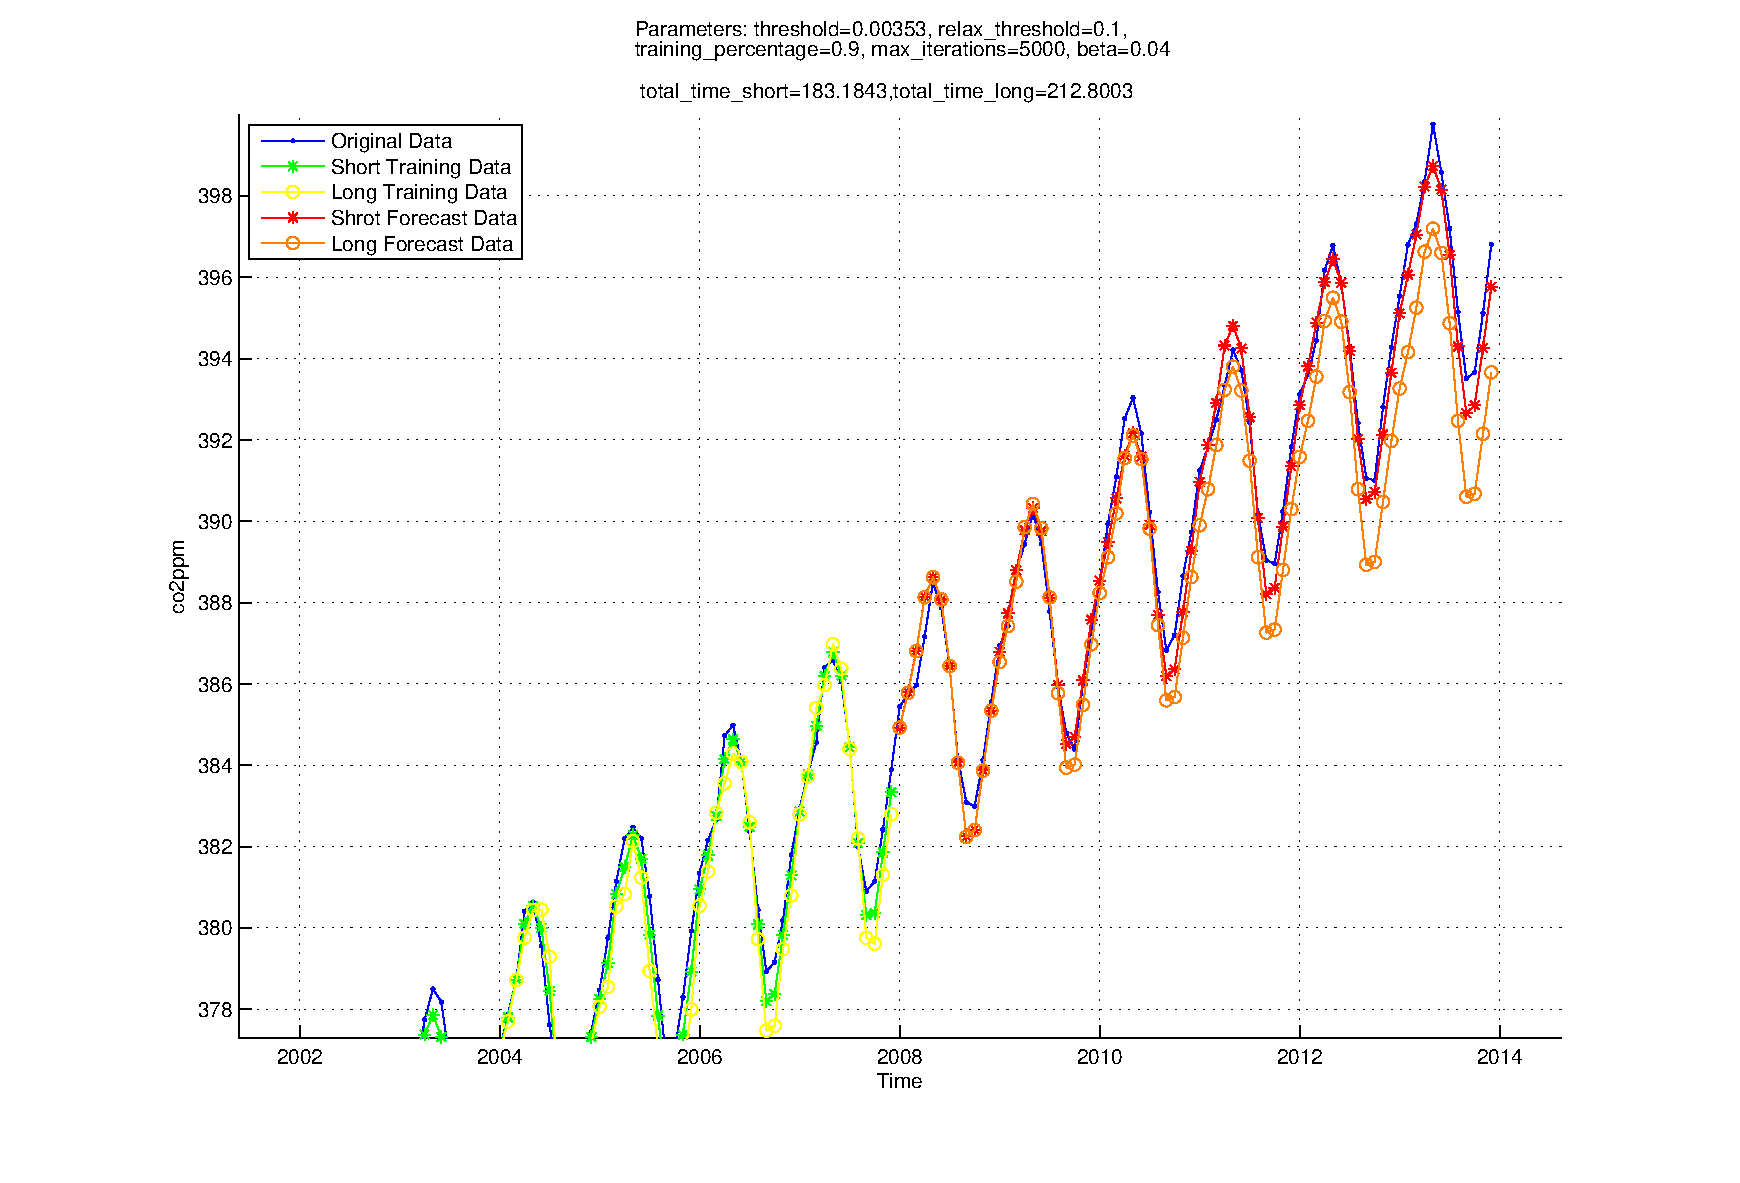
\includegraphics[width=\textwidth]{images/ais_visualization_2.eps}
  \caption{Visualization of the model (2)}
  \end{subfigure}%
   ~ %add desired spacing between images, e. g. ~, \quad, \qquad, \hfill etc.
  \begin{subfigure}[b]{0.51\textwidth}
    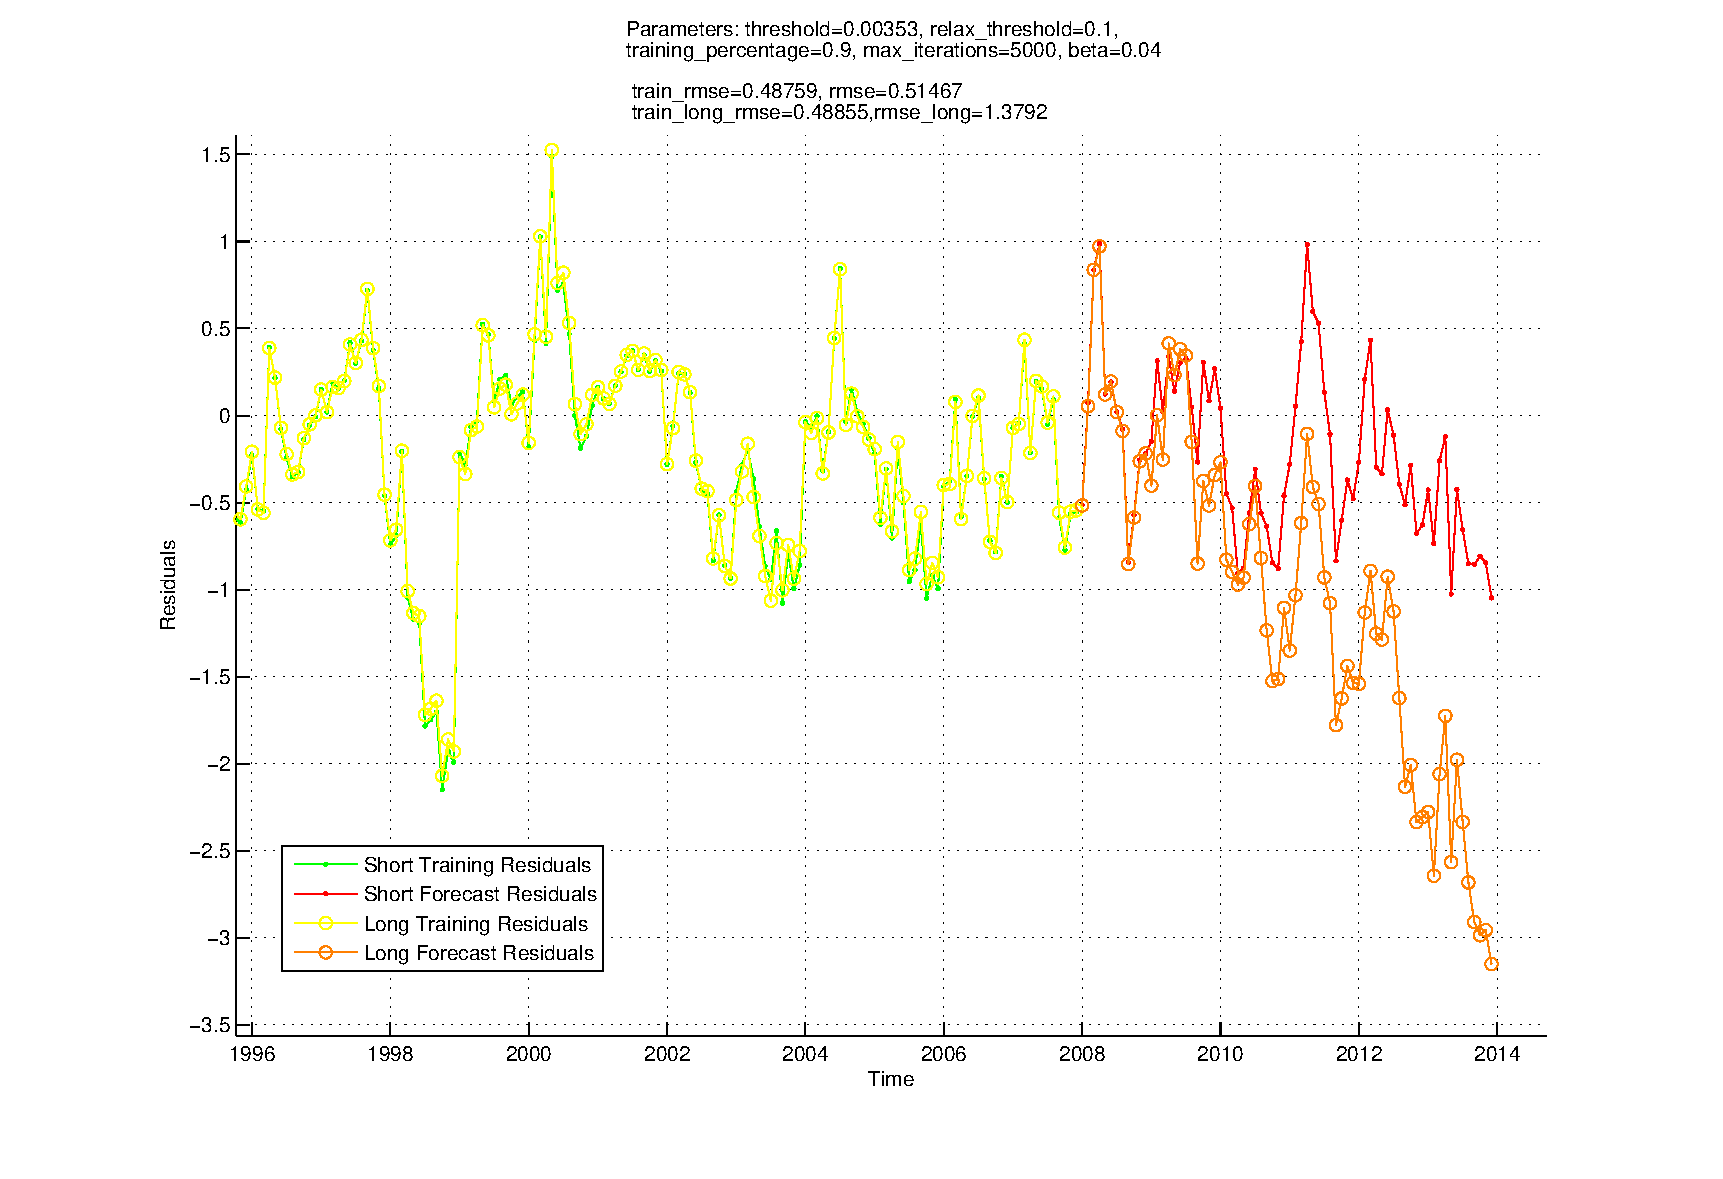
\includegraphics[width=\textwidth]{images/ais_residuals_2.eps}
  \caption{Visualization of the residuals (2)}
  \end{subfigure}

  \caption{AIS model}
\label{fig:ais_model}
\end{figure}

\begin{figure}
  \centering
  \begin{subfigure}[b]{0.51\textwidth}
     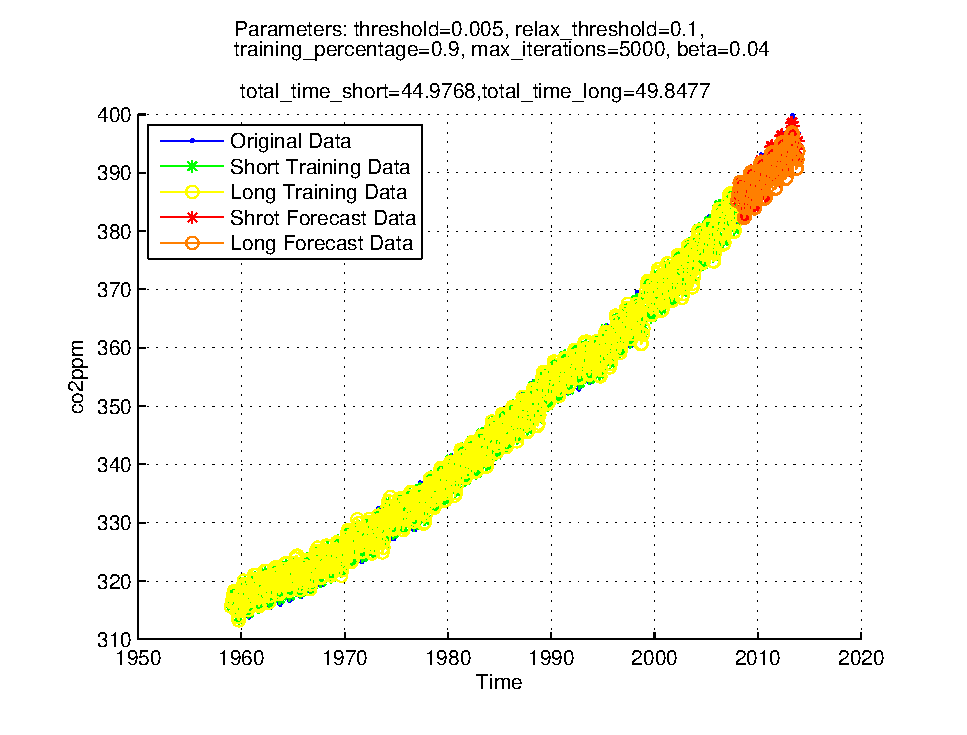
\includegraphics[width=\textwidth]{images/ais_visualization_0005.eps}
  \caption{Visualization of the model}
  \end{subfigure}%
   ~ %add desired spacing between images, e. g. ~, \quad, \qquad, \hfill etc.
  \begin{subfigure}[b]{0.51\textwidth}
    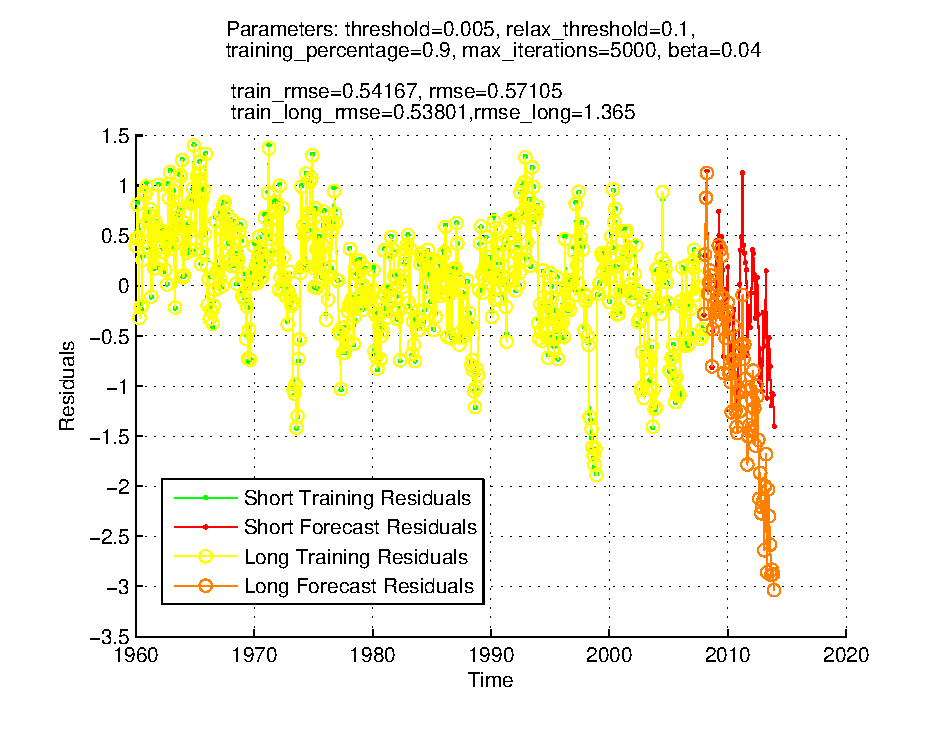
\includegraphics[width=\textwidth]{images/ais_residuals_0005.eps}
  \caption{Visualization of the residuals}
  \end{subfigure}

  \begin{subfigure}[b]{0.51\textwidth}
     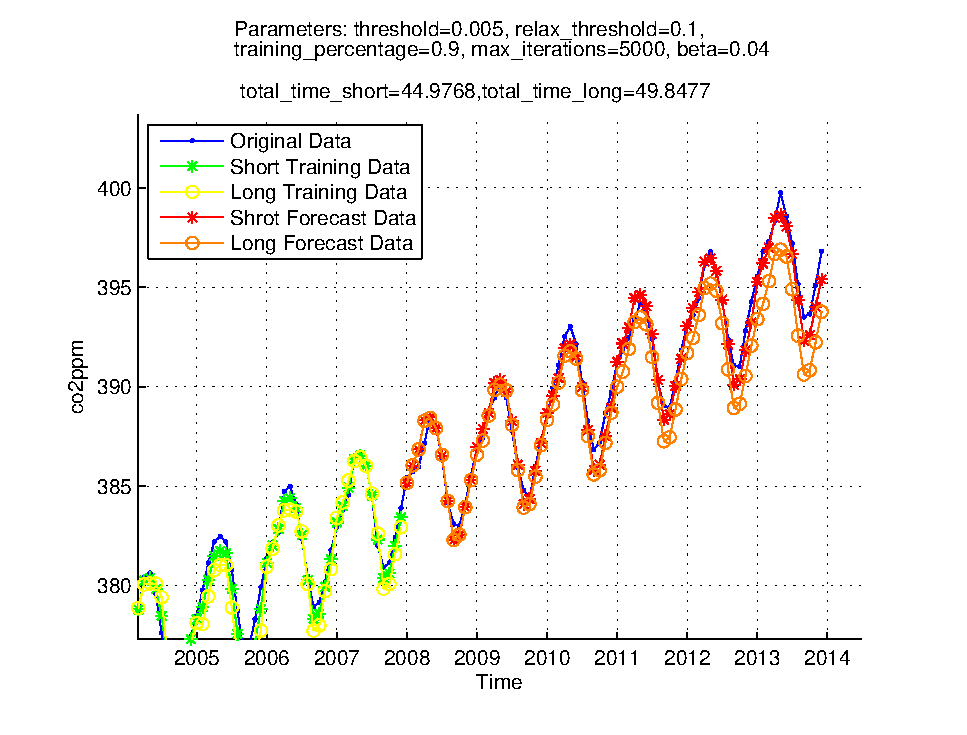
\includegraphics[width=\textwidth]{images/ais_visualization_0005_2.eps}
  \caption{Visualization of the model (2)}
  \end{subfigure}%
   ~ %add desired spacing between images, e. g. ~, \quad, \qquad, \hfill etc.
  \begin{subfigure}[b]{0.51\textwidth}
    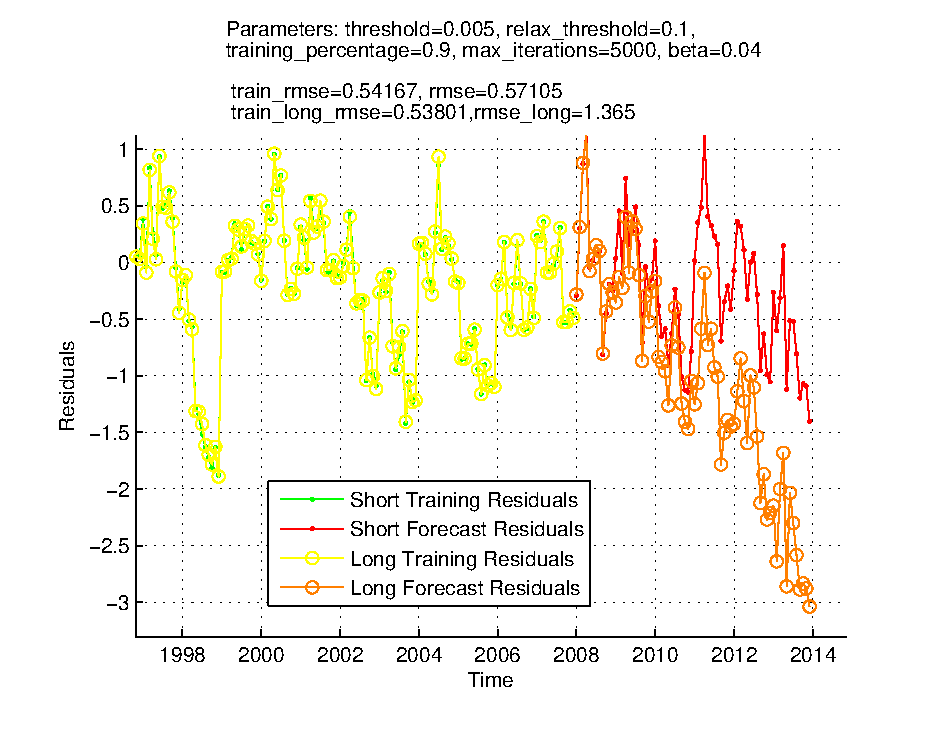
\includegraphics[width=\textwidth]{images/ais_residuals_0005_2.eps}
  \caption{Visualization of the residuals (2)}
  \end{subfigure}

  \caption{AIS model(2)}
\label{fig:ais_model_0005}
\end{figure}

\begin{table}
\begin{center}
  \begin{tabular}{|c|c|c|c|}
    \hline
    {\bf Model} & {\bf Parameters} & {\bf RMSE(train)} & {\bf RMSE(forecast)}\\ \hline \hline

	Linear Model & - & 3.183062 & 7.255561 \\ \hline

	Exponential Model & - & 2.212280 & 2.315118 \\ \hline

	\multirow{3}{*}{AIS Short model} &

	 threshold= 0.00353 & \multirow{3}{*}{0.48759} & \multirow{3}{*}{0.51467} \\ 
	 & relax\_threshold = 0.1 & & \\
	 & beta = 0.04 & & \\ \hline

	\multirow{3}{*}{AIS Long model} &

	 threshold= 0.00353 & \multirow{3}{*}{0.48855} & \multirow{3}{*}{1.3792} \\ 
	 & relax\_threshold = 0.1 & & \\
	 & beta = 0.04 & & \\ \hline

	\multirow{3}{*}{AIS Short model (2)} &

	 threshold= 0.005 & \multirow{3}{*}{0.54167} & \multirow{3}{*}{0.57105} \\ 
	 & relax\_threshold = 0.1 & & \\
	 & beta = 0.04 & & \\ \hline

	\multirow{3}{*}{AIS Long model (2)} &

	 threshold= 0.005 & \multirow{3}{*}{0.53801} & \multirow{3}{*}{1.365} \\ 
	 & relax\_threshold = 0.1 & & \\
	 & beta = 0.04 & & \\ \hline

\hline \hline
  \end{tabular}
\caption{The RMSE of the models}
\label{table:model_parameters}
\end{center}
\end{table}

\clearpage
\phantomsection \label{Bibliography}
\addcontentsline{toc}{section}{Bibliography}
\printbibliography

\newpage

\end{document}

